\begin{frame}[t]{Outlook: Many-Body Physics}
    \begin{textblock*}{.5\linewidth}(0cm, 0cm)
        
\includegraphics[width=\linewidth]{many_body}
        \textcite{astrakharchik2023many}
    \end{textblock*}

    \begin{textblock*}{.5\linewidth}(0.52\linewidth, 1.5cm)
        
\includegraphics[width=\linewidth]{phase_diagram}
        \textcite{astrakharchik2021ionic}
    \end{textblock*}
\end{frame}

\begin{frame}[t]{Outlook: Many-Body Physics}
    \begin{textblock*}{.55\linewidth}(0cm, 0cm)
        \begin{itemize}
            \item Weak and strong coupling both \textrightarrow $\delta m_{\mathrm{eff}}$
            \begin{itemize}
                \item[\textrightarrow] "'tickling"' at motional frequency to measure mass
            \end{itemize}
             \vspace{0.5cm}
            \item Weak coupling
            \begin{itemize}
                \item Able to resolve the shift?
                \item[\textrightarrow] Parametric excitation
            \end{itemize}
            \vspace{0.5cm}
            \item Strong coupling
            \begin{itemize}
                \item Do MBBSs live long enough?
            \end{itemize}
        \end{itemize}
        \small{\textcite{schmidt2020mass}}
    \end{textblock*}

    \begin{textblock*}{.45\linewidth}(0.55\linewidth, 0cm)
        
\includegraphics[width=0.7\linewidth]{para_res}
        \newline
        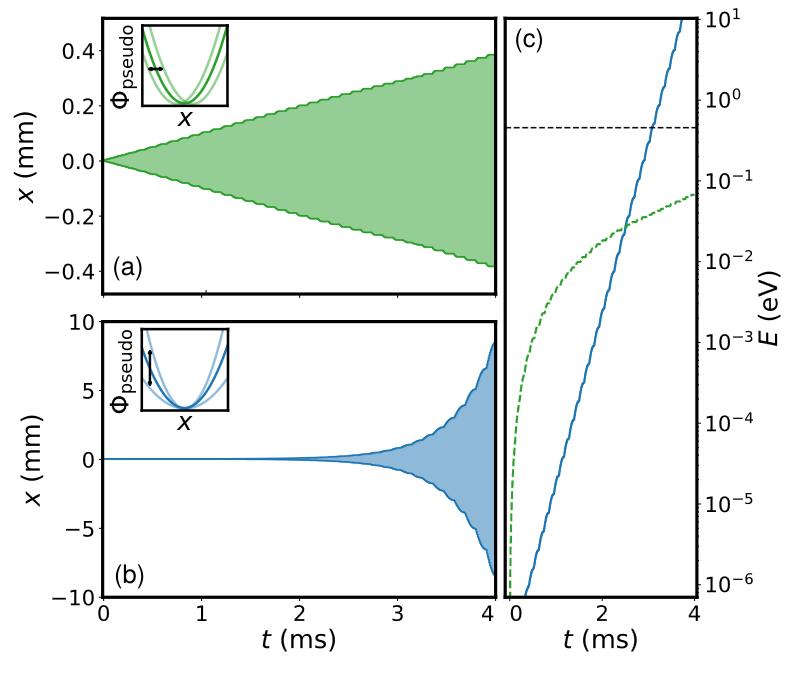
\includegraphics[width=0.7\linewidth]{parametric_time}
    \end{textblock*}
\end{frame}

\begin{frame}[t]{Outlook: Energy Dependance}

    \begin{textblock*}{.5\linewidth}(0cm, 0cm)
        \adjincludegraphics[width=0.8\linewidth, trim={0 0 {.5\width} 0},clip]{partial_waves}
    \end{textblock*}
\only<2>{
    \begin{textblock*}{.6\linewidth}(0.4\linewidth, 0cm)
        Experimental data in thulium:
        
\includegraphics[width=0.9\linewidth]{feshbach_temp}
        \textcite{Khlebnikov2019RandomTC}
    \end{textblock*}}
\end{frame}

\begin{frame}[t]{Outlook: Energy Dependance}
    \begin{itemize}
        \item Increase \Li{} bath temperature
        \begin{itemize}
            \item Evaporate to higher temp
                    \begin{itemize}
                        \item[\textrightarrow] more light \textrightarrow\, light assisted interaction?
                     \end{itemize}
            \item Adiabatic ramps?
        \end{itemize}
        \vspace{0.5cm}
        \item Increase \Ba{} energy
        \begin{itemize}
            \item Offset fields to increase micromotion
                \begin{itemize}
                \item[\textrightarrow] increase in rf power \textrightarrow\, rf association?
                \item[\textrightarrow] displacement \textrightarrow\, inhomogeneities?
                \end{itemize}
            \item Additional rf
                \begin{itemize}
                \item[\textrightarrow] increase in rf power \textrightarrow\, rf association?
                \end{itemize}
        \end{itemize}
    \end{itemize}
\end{frame}


\begin{frame}[t]{Outlook: All-Optical}
    \begin{itemize}
        \item Optical trapping of ions demonstrated for $t_{\mathrm{trap}} \gg t_{\mathrm{int}}$
        \vspace{0.5cm}
        \item No micromotion!
        \vspace{0.5cm}
        \item \ldots but even more light
            \begin{itemize}
                \item[\textrightarrow] light assisted interactions?
            \end{itemize}
    \end{itemize}
\end{frame}
